\textbf{COLUNI 2024 -- Questão 36}\par\medskip Observe a imagem e leia, atentamente, o texto a seguir:

\begin{center}
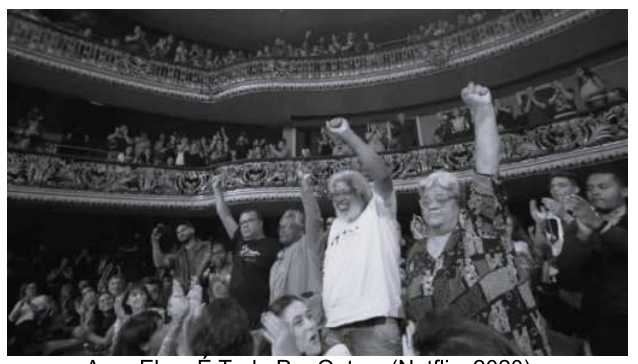
\includegraphics[width=0.45\linewidth,trim=0 12pt 0 0,clip]{static/simulados/coluni/figuras/2024/questao-36/figura-1.png}\\
AmarElo – É Tudo Pra Ontem (Netflix, 2020)
\end{center}

“Para que a gente esteja nesse lugar que foi negado aos nossos ancestrais, muitas pessoas suaram e sangraram no caminho. Se hoje a gente sorri dentro do Theatro Municipal, é porque algumas pessoas no auge da ditadura militar tiveram a coragem de se levantar contra o Estado brasileiro e seu racismo assassino e dizer que o país precisava reconhecer o protagonismo das pessoas de pele escura na sociedade brasileira. A nossa vitória não vale de nada se ela não anistiar o espírito de todas as pessoas que foram assassinadas durante cinco séculos de escravidão”. (Emicida. \textit{AmarElo: É Tudo Pra Ontem}. Netflix, 2020)

O texto acima faz parte do documentário \textit{AmarElo: é tudo pra ontem}, do rapper brasileiro Emicida. No caso, pouco antes da música \textit{Pantera Negra}, Emicida fez referência a um grupo de convidados especiais para seu show, realizado no Theatro Municipal de São Paulo. Eram pessoas (foto) que haviam participado do ato de fundação do Movimento Negro Unificado (MNU), ocorrido em 07 de julho de 1978, em plena ditadura civil-militar, justamente nas escadarias daquele mesmo Theatro Municipal.

Em relação aos Movimentos Negros no Brasil, no período entre a distensão da ditadura e o processo de redemocratização, é INCORRETO afirmar que:
\begin{enumerate}
\item a partir da rearticulação tecida desde a fundação do MNU, os Movimentos Negros apresentaram pautas
        que seriam discutidas na Constituição de 1988 e em legislações posteriores, relacionadas à população
        negra brasileira, tais como políticas de saúde, educação e cultura.
\item a presença dos fundadores do MNU no documentário se refere à maneira como a população negra se
        articulou politicamente, ao longo do tempo, sendo responsável por avanços em direitos-civis, vivenciados
        hoje, mesmo com muito por se fazer.
\item a reação da ditadura à fundação do MNU foi dura, fazendo com que houvesse adesões ao movimento
        especificamente a partir de 1988, ano do centenário da abolição e de promulgação da Constituição
        Cidadã, o que desenhou uma conjuntura propícia para se discutir o racismo no Brasil.
\item a partir do início da década de 1980, o MNU ampliou a divulgação de suas principais reivindicações,
        dentre as quais estavam a desmistificação da democracia racial brasileira e a introdução da História da
        África e do Negro no Brasil nos currículos escolares.
\end{enumerate}
